%----------------------------------------------------------------------------------------
% Literature review
%----------------------------------------------------------------------------------------

\section{Reproducing Kernel Hilbert Space} 

\subsection{Hilbert Space}
The theory of Hilbert space was initiated by David Hilbert. \citet{debnath2005introduction} provides a detailed explanation of Hilbert space $\mathcal{H}$. It is defined as an inner product space that is complete and separable with respect to the norm defined by the inner product.
An example of a defined norm in Hilbert space (i.e, the space $L_2$ of square-integrable functions) can be 
\begin{equation*}
    \parallel f \parallel = \left(\int_a^b f^2(t)dx\right)^\frac{1}{2}.
\end{equation*}
A normed space is a vector space $N$ on which a norm is defined. A non-negative function $\parallel\cdot\parallel$ is a norm if and only if $\forall f,g\in N$ and $\alpha\in\mathbb{R}$:
\begin{itemize}
    \item $\parallel f \parallel \geq 0$ and $\parallel f\parallel=0$ iff $f=0$;
    \item $\parallel f+g \parallel \leq \parallel f \parallel + \parallel g \parallel$;
    \item $\parallel \alpha f\parallel=\mid \alpha \mid \parallel f \parallel$
\end{itemize}
Examples of inner product $<a,b>$ in a Hilbert space are
\begin{itemize}
    \item a usual dot product: $<a,b>=a'b=\sum_i a_i b_i$.
    \item a kernel product: $<a,b>=k(a,b)=\psi(a)'\psi(b)$, where $\psi(a)$ may have infinite dimensions.
\end{itemize} 

\subsection{Introduction to Kernel}
\subsubsection{Feature map}
The motivation of the kernel method is simple. Imagine there are some blue dots and red dots on a vector space $\mathcal{R}^2$ and 
we want to separate them by color. As it is shown in the left-hand side figure, it is difficult to divide them through a straight 
line. However, we may be able to separate them easily by mapping each dot into a high-dimension feature space. The figure below 
shows how the feature map works:
\begin{figure}[htpb!]
    \centering
    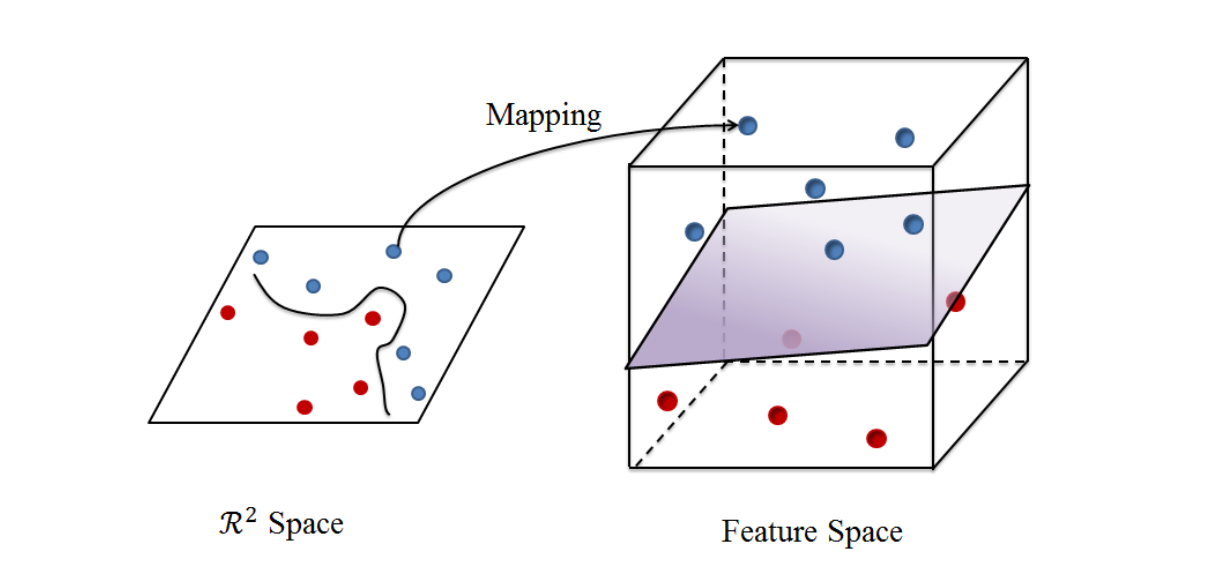
\includegraphics[width=0.7\textwidth]{figure/Mapping.png}
\end{figure}
\\ \\
Let's now use a simple example to illustrate the idea of a feature map. 
we set two vectors $\textbf{x}=\begin{bmatrix}x_1&x_2\end{bmatrix}$ and $\textbf{y}=\begin{bmatrix}y_1&y_2\end{bmatrix}$ in a two-dimension space.
Tow functions $\phi(x)$ and $\phi(y)$ are defined as:
\begin{equation*}
    \phi(x)=\begin{bmatrix}
        x_1x_1&x_1x_2&x_2x_1&x_2x_2
    \end{bmatrix}
\end{equation*}
\begin{equation*}
    \phi(y)=\begin{bmatrix}
        y_1y_1&y_1y_2&y_2y_1&y_2y_2
    \end{bmatrix}
\end{equation*}
We are now successfully mapping them into a four-dimension feature space. 
To write the above example in a general form of linear regression, we first set an equation where $\phi(\cdot)\in\mathcal{R}^m$ and $\phi(x)$ is defined as the mapping function. Note that we assume there is a linear relation between $y$ and $\phi(x)$:
\begin{align}
    y&=\phi(x)^\top w \notag\\
     &= \begin{bmatrix}
        \phi_1(x)\cdots\phi_m(x)
        \end{bmatrix} w
\end{align}
$Y$ and $\Phi$ in generalization is defined by:
\begin{equation}
    Y=\begin{bmatrix}
         y_1&\cdots&y_n
      \end{bmatrix}^\top 
\end{equation}
\begin{align}
    \Phi&=\begin{bmatrix}
           \phi(x_1)&\cdots&\phi(x_n) 
          \end{bmatrix}^\top \notag\\
        &=\begin{bmatrix}
           \phi_1(x_1)&\cdots&\phi_m(x_1)\\
           \vdots&\vdots&\vdots \\
           \phi_1(x_n)&\cdots&\phi_m(x_n)
          \end{bmatrix}
\end{align}
Recall the regularized risk minimization problem of ridge regression. In this case, it can be re-written as:
\begin{align*}
  w{*}&=\underset{w}{\operateorname{argmin}}\sum_{i=1}^n(y_i-\phi(x_i)^\top w)^2+\lambda\parallel w \parallel_2^2 \\
      &=\underset{w}{\operateorname{argmin}}\parallel Y-\Phi w\parallel_2^2+\lambda\parallel w\parallel_2^2
\end{align*}
The least-square solution can also be re-defined by:
\begin{equation}
    w{*}=(\Phi^\top\Phi+\lambda I)^{-1}\Phi^\top Y
\end{equation}
Then we replace $w{*}$ with $(\Phi^\top \Phi+\lambda I)^{-1}\Phi^\top$ in $y=\phi(x)^\top w$, we get:
\begin{align}
    y_w{*} (x)&=\phi(x)^\top w{*}\notag\\
            &=\phi(x)^\top(\Phi^\top \Phi+\lambda I)^{-1}\Phi^\top Y\notag\\
            &=\underbrace{\phi(x)^\top \Phi^\top}_\text{$1\times n$}(\underbrace{\Phi\Phi^\top}_\text{$n\times n$}+\lambda I)^{-1}Y\\
            &\text{using that} (\Phi^\top \Phi+\lambda I)^{-1}\Phi^\top=\Phi^\top(\Phi\Phi^\top+\lambda I)^{-1}\notag
\end{align}


\subsubsection{Kernel Method}
In most cases, it is surprisingly difficult to know and calculate the feature function after mapping. We want to avoid computing $\phi(x)$ in an explicit way, 
especially when $m$ is very large. Therefore, we define a kernel function:
\begin{equation*}
    [\Phi\Phi^\top]_{i,j}=\phi(x_i)^\top \phi(x_j)=K(x_i,x_j)
\end{equation*}
\begin{equation}
    [\phi(x)^\top\Phi^\top]_j=\phi(x)^\top\phi(x_j)=K(x,x_j)
\end{equation}
This is simply the intuition of using the kernel method. For example, the Gaussian kernel is
\begin{equation*}
    k(x_i, x_j) = e^\frac{-\parallel x_i - x_j \parallel}{\sigma^2},
\end{equation*}
Gaussian kernel meaning the similarity between two points where $\parallel x_i - x_j \parallel$ is the Euclidean distance between $x_i$ and $x_j$, and $\sigma^2 \in \mathbb{R}^+$ is the bandwidth of the kernel function. As shown in \citet{hofmann2008kernel}, it has the following properties:\\
for $k: \mathcal{X} \times \mathcal{X} \rightarrow \mathbb{R}$ is a kernel if
\begin{itemize}
    \item $k$ is symmetric: $k(x,y) = k(y,x)$.
    \item $k$ is positive semi-definite, meaning that $\sum_{i} \sum_{j} \alpha_i \alpha_j k(x_i,x_j)\geq0, \forall \alpha_i, \alpha_j \in \mathbb{R}, x \in \mathbb{R}^\mathbb{D}, \mathbb{D} \in \mathbb{Z}^+$. 
    \item We define the corresponding kernel matrix as the matrix $K$ with entries $k_{ij}=k(x_i,x_j)$, the sencond property of $k$ is equivalent to saying that $\textbf{a}'K \textbf{a}\geq 0$.
\end{itemize}
Now we can define a function k: $\mathcal{X} \times \mathcal{X}  \rightarrow \mathbb{R}$ is a kernel if and 
only if there exists a Hilbert space $\mathcal{H}$ and a map $\phi: \mathcal{X}\rightarrow\mathcal{H}$ such that $k(x,y)=\langle\phi(x),\phi(y)\rangle$. \\
Recall the simple example above, instead of computing the inner product of $\langle\phi(x),\phi(y)\rangle$, we can define 
a corresponding kernel function $K(\textbf{x},\textbf{y})=\langle\textbf{x},\textbf{y}\rangle^2$. It can be easily proofed that $K(\textbf{x},\textbf{y})$ is the same as $\langle\phi(\textbf{x}),\phi(\textbf{y})\rangle$:
\begin{align*}
    K(\textbf{x},\textbf{y})&=\langle\textbf{x},\textbf{y}\rangle^2\\
                            &=(x_1y_1+x_2y_2)^2\\
                            &=x_1^2y_1^2+2x_1y_2x_2y_1+x_2^2y_2^2\\
                            &=\langle\phi(\textbf{x}),\phi(\textbf{y})\rangle
\end{align*}

\subsection{Reproducing Kernel Hilbert Space}
Consider a Hilbert space $\mathcal{H}$ full of real-valued functions from $\mathcal{X}$ to $\mathbb{R}$, and a mapping $\Phi: \mathcal{X}\rightarrow\mathbb{R}^\chi$ defined as $x\rightarrow\Phi(x)=k_x=k(\cdot , x)$. A function $k:\mathcal{X}\times\mathcal{X}\rightarrow\mathbb{R}$ is a 
reproducing kernel of $\mathcal{H}$, and $\mathcal{H}$ is a reproducing kernel Hilbert space, if:
\begin{itemize}
    \item $\forall x \in\mathcal{X}$, $k(\cdot, x)\in\mathcal{H}$,
    \item $\forall x \in\mathcal{X}$, $f\in\mathcal{H}$, $\langlef(\cdot),k(\cdot,x)\rangle_\mathcal{H}=f(x)$, which is the reproducing property.
\end{itemize}
To be more intuitive, a Reproducing Kernel Hilbert Space is a Hilbert space $\mathcal{H}$ with a reproducing kernel whose span is dense in $\mathcal{H}$. Equivalently, an RKHS can be defined as a Hilbert space of valid functions with all evaluation functionals bounded and linear. 

\subsection{Representer Theorem}
In the previous section, we have learned that there is always a pair of $(\mathcal{X},k)$ as a Hilbert space or a subset of that space whenever the input domain $\mathcal{X}$ exists. Such a fact means that we are able to study the various data structures in Hilbert spaces. 
In the practical world, however, it is extremely difficult to study many popular kernels since their Hilbert spaces are known to be infinite-dimensional in almost every case. Especially for the purpose of machine learning, we usually prefer to solve an optimization problem in a finite-dimensional space. \\
This is where the representer theorem is useful. It contributes to simplifying the regularized risk-minimization problem by reducing the infinite-dimensional space to a finite-dimensional vector of optimal coefficients and provides provisions for kernels in training data in machine learning.\\
Suppose we are given a nonempty set $\mathcal{X}$, a positive definite real-valued kernel $k$ on $\mathcal{X}\times\mathcal{X}$, a training sample $(x_1,y_1),\dots,(x_m,y_m)\in\mathcal{X}\times\mathbb{R}$, a strictly monotonically increasing real-valued function $f$ on $[0,\infty[$. As explained in \citet{scholkopf2001generalized}, we can find the function $f^{*}$ in the RKHS $\mathcal{H}$ satisfying:
\begin{equation*}
    \mathcal{J}(f^{*})=\underset{f\in\mathcal{H}}{min}\mathcal{J}(f),
\end{equation*}
where 
\begin{equation*}
    \mathcal{J}(f)=L_y(f(x_1),\cdots,f(x_n))+\Omega(\parallel f \parallel_\mathcal{H}^2).
\end{equation*}
Note that $\Omega$ is a non-decreasing regularizer and $y$ is a vector of $y_i$. \\
In the simplest form of machine learning, in order to predict $x$, the algorithm collects the samples in the training set $\mathcal{X}$ that are similar to $x$, 
and then takes the weighted value of these samples as the predict value of $x$. Here comes the questions:
\begin{itemize}
    \item How to measure the similarity between samples?
    \item How to weigh the value of each sample?
\end{itemize} 
In general, the higher the similarity of the sample to our point of interest $x$, the more the sampling weights. To evaluate the similarity between two observations, 
a kernel is defined as a function of two input patterns $k(x_i, x_j)$, mapping onto a real-valued output. \citet{hofmann2008kernel} wrote that the advantage of using such a kernel as a similarity measure is that it allows us to construct algorithms in dot product spaces.\\
The representer theorem is that the solution to $\underset{f\in\mathcal{H}}{min}[L_y(f(x_1),\cdots,f(x_n))+\Omega(\parallel f \parallel_\mathcal{H}^2)]$ can 
be written in a simpler version, which takes the form $f^{*}=\sum_{i=1}^n\alpha_i k(x_i,\cdot)$, where $\alpha_i$ the weighted value of each sample and $k$ is the similarity measure. If $\Omega$ is strictly increasing, all solutions apply to this form. 


\subsection{Example Using Representer Theorem--Kernel Ridge Regression}
Suppose we are given empirical data $(y_1,x_1),\dots,(y_n,x_n)$, where $i = 1, \dots, N$. Assume $y=g(x)$ in RKHS. We want to estimate the function $g(\cdot)$ to minimize
\begin{equation}
    \underset{g\in\mathcal{H}}{min}\sum_{i=1}^N(y_i-g(x_i))^2+\Omega\parallel g\parallel_\mathcal{H}^2
\end{equation}
In order to avoid extremely high variance, we impose an additional assumption 
that a smoother curve with fewer oscillations is preferred. We utilize regularization to simplify the function and satisfy the additional assumption by adding a penalty term $\Omega$. Luckily, the representer theorem already tells us that the least squared problem always has a solution of the form 
\begin{equation}
    g(\cdot)^{*}=\sum_{i=1}^N\alpha_i k(\cdot,x_i),
\end{equation}
and according to reproducing property of RKHS, we have
\begin{equation}
    g(x)=\langle g(\cdot), k(\cdot, x)\rangle_\mathcal{H}.
\end{equation}
Also, it is obvious that
\begin{equation}
    \parallel g \parallel^2=\langle g(\cdot),g(\cdot)\rangle.
\end{equation}
We then substitute $(9)$, $(10)$ for $(7)$,
\begin{equation*}
    \underset{g\in\mathcal{H}}{min}\sum_{i=1}^N(y_i-\langle g(\cdot),k(\cdot, x)\rangle)^2+\Omega\langle g(\cdot),g(\cdot)\rangle,
\end{equation*}
and plug $(8)$ in $(7)$ and get
\begin{equation*}
    \underset{\alpha}{min}\sum_{i=1}^N(y_i-\langle \sum_{j=1}^N\alpha_j k(\cdot, x_j),k(\cdot,x_i)\rangle)^2+\Omega\langle \sum_{i=1}^N\alpha_i k(\cdot, x_i),k(\cdot,x_j)\rangle\\
\end{equation*}
\begin{equation*}
    \Rightarrow\underset{\alpha}{min}\sum_{i=1}^N(y_i-\sum_{j=1}^N\alpha_j k(x_j,x_i))^2+\Omega\sum_{i=j}^N\sum_{i=1}^N\alpha_j\alpha_i k(x_i,x_j)
\end{equation*}
Remember the corresponding kernel matrix as the matrix $K$ with entries $k_{ij}=k(x_i,x_j)$ is equivalent to saying that $\textbf{a}'K \textbf{a}\geq 0$, we can then rewrite the kernel ridge regression as:
\begin{equation*}
    \parallel y_i-K \textbf{a}\parallel^2+\Omega \textbf{a}' K\textbf{a}.
\end{equation*}
By differentiation and setting the equation $(9)$ to zero, we get:
\begin{equation}
    \alpha^{*}=(K+\Omega I_n)^{-1}y.
\end{equation}


\subsection{Example of Solving the Kernel Function}
In this paper, we study in the RKHS $\mathcal{H} = \mathcal{H}_{\omega ,\delta}$ consisting of differentiable functions $ h : [0, \infty ) \to \mathbb{R}$ of the form $h(x) = \int_{0}^{x} h'(t) dt$ with continuous derivatives, $h'(x) = h'(0) + \int_{0}^{x} h''(t)dt $ for integrable $h''$, and with finite norm 
\begin{equation}
\langle h, h\rangle = \parallel h \parallel_{\omega ,\delta} = (\int_{0}^{\infty} (\delta h'(x)^2 + (1 - \delta)h''(x)^2)\omega (x)dx)^{\frac{1}{2}}
\end{equation}
for some measurable weight function $\omega : [0, \infty) \to [1, \infty)$ and shape parameter $\delta \in (0,1)$. With additional assumption in the research paper's appendix A.2, we can extend it to the case $\delta \in \{ 0, 1\}$. \\
The Lemma 3 assumes that for any fixed $y \ge 0$, exists a solution $\phi$ of the linear differential equation 
\begin{equation}
\delta \phi \omega - (1-\delta )(\phi ' \omega)' = 1_{[0,y]}
\end{equation}
and for $\psi  \in \mathcal{H}_{\omega, \delta}, \psi (x) = \int_{0}^{x} \phi (t)dt$, then for $h \in \mathcal{H}_{\omega, \delta}$ with $h'(x) = 0$ for $x > n$ for some finite $n$, we can write 
\begin{equation}
\langle \psi , h\rangle_{\omega, \delta} = \int_{0}^{\infty} (\delta \psi '(x) h'(x) + (1-\delta )\psi '' h''(x))\omega (x)dx
\end{equation}
according to the definition for any $h \in \mathcal{H}_{\omega,\delta}$. The assumption of sloution exists and Lemma 4 could give us that $\langle \psi , h\rangle = h(y)$ which implies that $k(\cdot , y) = \psi$ by the reproducing property. Then  $k(x , y) = \psi (x)$, and remind that $\psi (x) = \int_{0}^{x} \phi (t)dt$, then we can find the form of $k(x,y)$ if we know the form of $\phi$, and we could solve $\phi$ by giving different value of $\delta$ and $\omega$. Below is an example of how to solve the research paper's equation 8. \\
In the research paper, the weight function $\omega (x) = e^{\alpha x}$, if $\alpha = 0, \delta = 1$, then $ \phi = 1_{[0,y]}$, and $k(x,y) = \psi (x) = \int_{0}^{x} 1_{[0,y]} dt = min\{x, y\}$. 
